\documentclass[tikz, border=2pt]{standalone}
\usepackage{amsmath}

\begin{document}
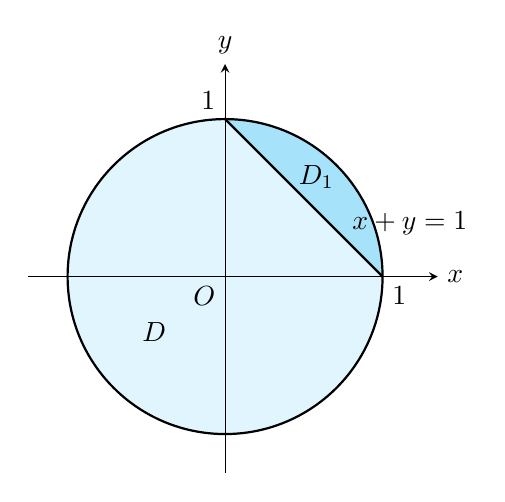
\begin{tikzpicture}[scale=2, >=stealth]
    % Unit disk split by x+y=1.
    \fill[cyan!12] (0,0) circle (1);
    \fill[cyan!35]
    (1,0)
    arc[start angle=0,end angle=90,radius=1]
    -- cycle;

    \draw[->] (-1.25,0) -- (1.35,0) node[right] {$x$};
    \draw[->] (0,-1.25) -- (0,1.35) node[above] {$y$};

    \draw[thick] (0,0) circle (1);
    \draw[thick] (1,0) -- (0,1);

    \node[below left] at (0,0) {$O$};
    \node[below right] at (1,0) {$1$};
    \node[above left] at (0,1) {$1$};
    \node[above left] at (1.6,0.2) {$x+y=1$};
    \node at (0.58,0.63) {$D_1$};
    \node at (-0.45,-0.35) {$D$};
\end{tikzpicture}
\end{document}
